\documentclass[a4paper,11pt,openright]{report}
\setlength{\parindent}{0pt} % set noindent for entire file

\usepackage[utf8]{inputenc}
\usepackage[a4paper,top=20mm,bottom=25mm,left=10mm,right=15mm]{geometry}
\usepackage{xcolor,graphicx}
\usepackage{amsmath}
\usepackage{setspace}
\usepackage{sectsty}
\usepackage{etoolbox}
\usepackage{enumitem}
\usepackage{listings}
\usepackage{times}

\graphicspath{ {/home/saran/Analytics/May_04/} }

\lstdefinestyle{mystyle}{
	backgroundcolor=\color{white},
	basicstyle=\ttfamily\footnotesize,
	breakatwhitespace=false,
	breaklines=true,
	captionpos=b,
	keepspaces=true,
	showspaces=false,
	showstringspaces=false,
	showtabs=false,
	tabsize=4
}

\lstset{style=mystyle}

\begin{document}
\singlespacing
\pagestyle{plain}

\begin{center}
\textbf{Assignment Normal Distribution} \\
Date: 04/05/2020 \hspace{2mm} Name: D.Saravanan
\end{center}

\vspace{10px}

\begin{enumerate}

\item[1.] Find the area under the standard normal curve which lie 

A normal distribution in a variate $X$ with mean $\mu$ and variance $\sigma^{2}$ is
a statistic distribution with probability density function 
\begin{equation*}
P(x) = \frac{1}{\sigma \sqrt{2\pi}} e^{-(x-\mu)^{2}/(2\sigma^{2})} 
\end{equation*}

The standard normal distribution is given by taking $\mu = 0$ and $\sigma^{2} = 1$ in 
a general normal distribution. An arbitrary normal distribution can be converted to a
standard normal distribution by changing variables to $Z \equiv (X-\mu)/\sigma$, so
$dz = dx/\sigma$, yielding
\begin{equation*}
P(x) dx = \frac{1}{\sqrt{2\pi}} e^{-z^{2}/2} dz
\end{equation*}

The normal distribution function $\Phi(z)$ gives the probability that a standard normal
variate assumes a value in the interval $[0,z]$,
\begin{equation*}
\Phi(z) \equiv \frac{1}{\sqrt{2\pi}} \int_{0}^{z} e^{-x^{2}/2} dx
\end{equation*}

The normal distribution is the limiting case of a discrete binomial distribution
$P_{p}(n|N)$ as the sample size $N$ becomes large, in which case $P_{p}(n|N)$ is normal with
mean $\mu = N p$ and variance $\sigma^{2} = N p(1-p)$. \\

The distribution $P(x)$ is properly normalized since 
\begin{equation*}
\int_{-\infty}^{\infty} P(x) dx = 1
\end{equation*}

The cumulative distribution function, which gives the probability that a variate will assume
a value $\leq x$, is then the integral of the normal distribution,
\begin{equation*}
\begin{split}
D(x) & \equiv \int_{-\infty}^{x} P(x^{'}) dx^{'} \\
& = \frac{1}{\sigma\sqrt{2\pi}} \int_{-\infty}^{x} e^{-(x^{'}-\mu)^{2}/(2\sigma^{2})} dx^{'}
\end{split}
\end{equation*}

Normal distributions have many convenient properties, so random variates with unknown
distributions are often assumed to be normal. It is often a good approximation due to the
central limit theorem. This theorem states that the mean of any set of variates with any 
distribution having a finite mean and variance tends to the normal distribution. \\

\pagebreak

\begin{enumerate}

\item[a)] To the right of $Z = 2.70$
\begin{equation*}
P(Z > 2.70) = \frac{1}{\sqrt{2\pi}} \int_{2.70}^{\infty} e^{-z^{2}/2} dz = 0.00347
\end{equation*}

Program:
\lstinputlisting[language=Python]{integration1a.py}
Output:
\lstinputlisting{output11a.txt}

Program:
\lstinputlisting[language=Python]{snormscipya.py}
Output:
\lstinputlisting{output12a.txt}

%figure_1
\begin{figure}[ht!]
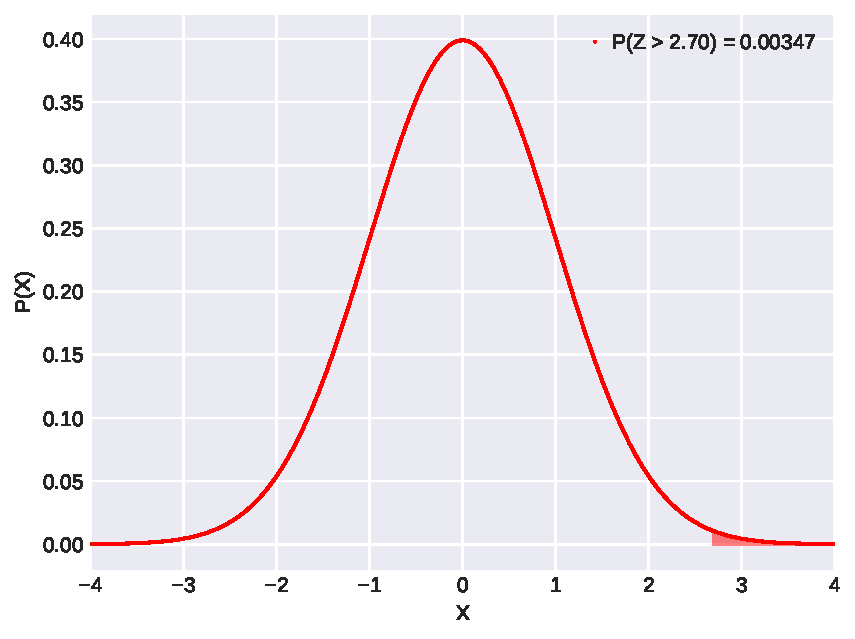
\includegraphics[width=14cm,height=7cm,keepaspectratio]{norm1a.pdf}
\centering
\end{figure}

\pagebreak

\item[b)] To the left of $Z = 1.73$
\begin{equation*}
P(Z < 1.73) = \frac{1}{\sqrt{2\pi}} \int_{-\infty}^{1.73} e^{-z^{2}/2} dz = 0.95818
\end{equation*}

Program:
\lstinputlisting[language=Python]{integration1b.py}
Output:
\lstinputlisting{output11b.txt}

Program:
\lstinputlisting[language=Python]{snormscipyb.py}
Output:
\lstinputlisting{output12b.txt}

%figure_2
\begin{figure}[ht!]
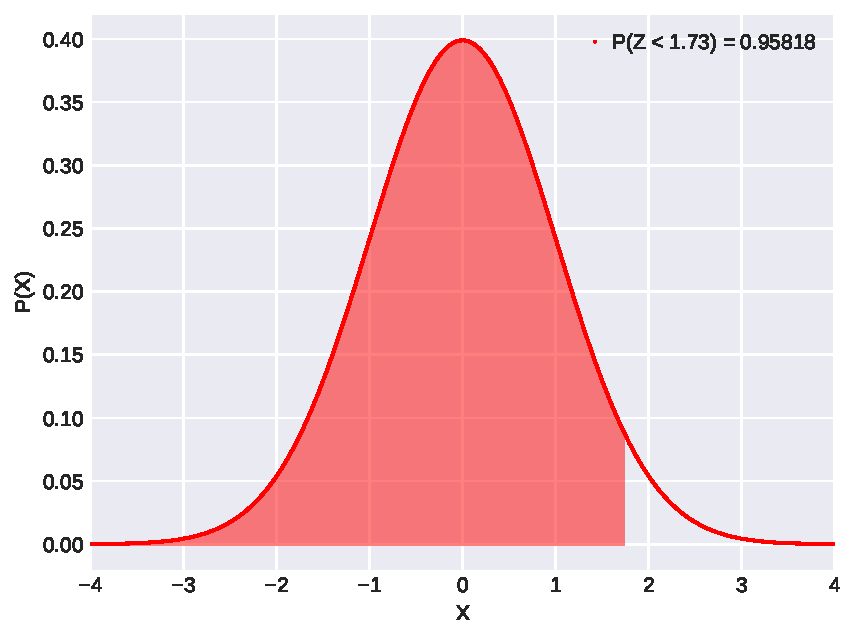
\includegraphics[width=14cm,height=7cm,keepaspectratio]{norm1b.pdf}
\centering
\end{figure}

\pagebreak

\item[c)] To the right of $Z = -0.66$
\begin{equation*}
P(Z > -0.66) = \frac{1}{\sqrt{2\pi}} \int_{-0.66}^{\infty} e^{-z^{2}/2} dz = 0.74537
\end{equation*}

Program:
\lstinputlisting[language=Python]{integration1c.py}
Output:
\lstinputlisting{output11c.txt}

Program:
\lstinputlisting[language=Python]{snormscipyc.py}
Output:
\lstinputlisting{output12c.txt}

%figure_3
\begin{figure}[ht!]
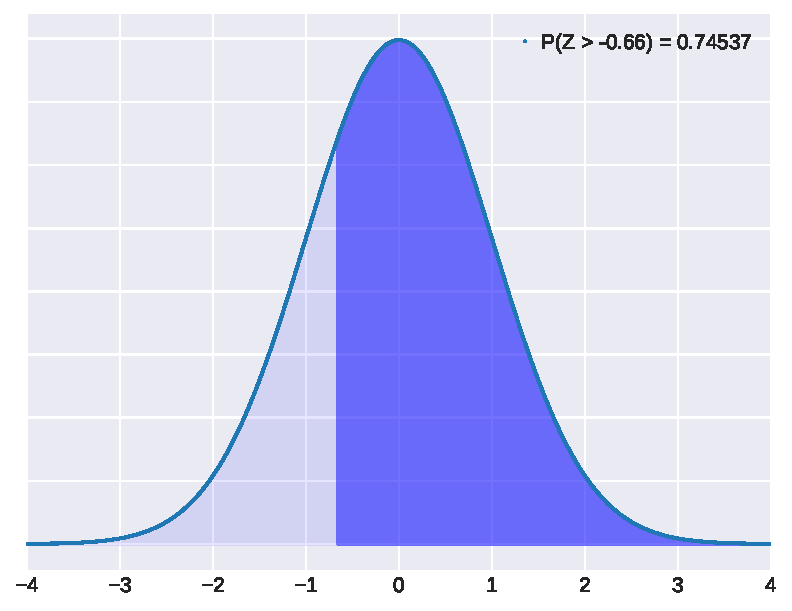
\includegraphics[width=14cm,height=7cm,keepaspectratio]{norm1c.pdf}
\centering
\end{figure}

\pagebreak

\item[d)] To the left of $Z = -1.88$
\begin{equation*}
P(Z < -1.88) = \frac{1}{\sqrt{2\pi}} \int_{-\infty}^{-1.88} e^{-z^{2}/2} dz = 0.03005
\end{equation*}

Program:
\lstinputlisting[language=Python]{integration1d.py}
Output:
\lstinputlisting{output11d.txt}

Program:
\lstinputlisting[language=Python]{snormscipyd.py}
Output:
\lstinputlisting{output12d.txt}

%figure_4
\begin{figure}[ht!]
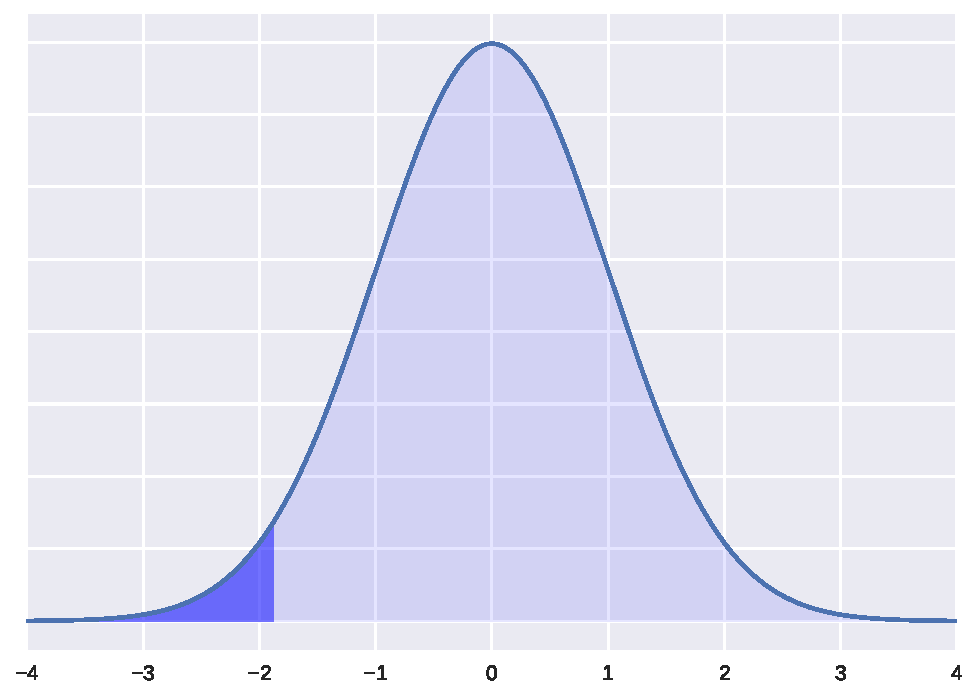
\includegraphics[width=14cm,height=7cm,keepaspectratio]{norm1d.pdf}
\centering
\end{figure}

\pagebreak

\item[e)] Between $Z = -0.90$ and $Z = -1.85$
\begin{equation*}
P(-1.85 < Z < -0.90) = \frac{1}{\sqrt{2\pi}} \int_{-1.85}^{-0.90} e^{-z^{2}/2} dz = 0.15190 
\end{equation*}

Program:
\lstinputlisting[language=Python]{integration1e.py}
Output:
\lstinputlisting{output11e.txt}

Program:
\lstinputlisting[language=Python]{snormscipye.py}
Output:
\lstinputlisting{output12e.txt}

%figure_5
\begin{figure}[ht!]
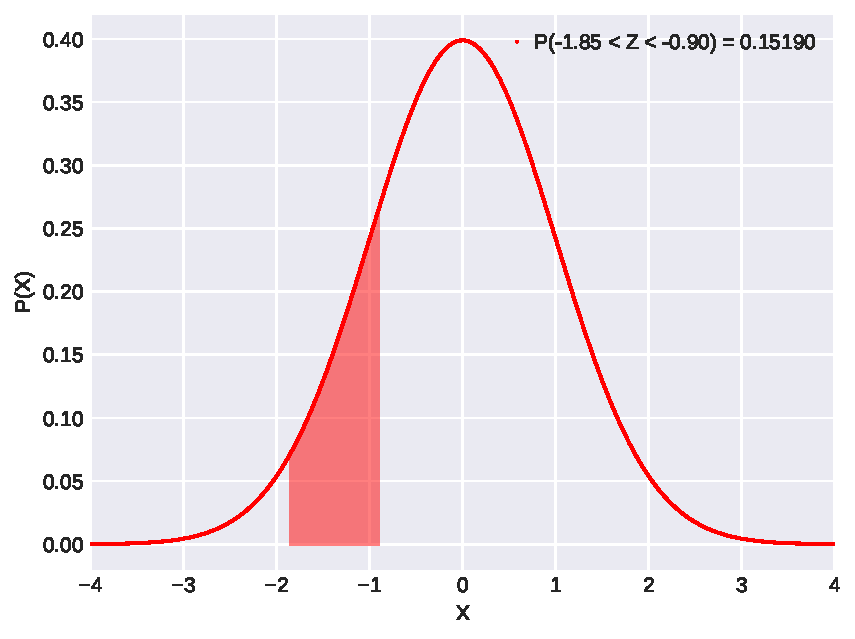
\includegraphics[width=14cm,height=7cm,keepaspectratio]{norm1e.pdf}
\centering
\end{figure}

\pagebreak

\item[f)] Between $Z = -1.45$ and $Z = 1.45$
\begin{equation*}
P(-1.45 < Z < 1.45) = \frac{1}{\sqrt{2\pi}} \int_{-1.45}^{1.45} e^{-z^{2}/2} dz = 0.85294
\end{equation*}

Program:
\lstinputlisting[language=Python]{integration1f.py}
Output:
\lstinputlisting{output11f.txt}

Program:
\lstinputlisting[language=Python]{snormscipyf.py}
Output:
\lstinputlisting{output12f.txt}

%figure_6
\begin{figure}[ht!]
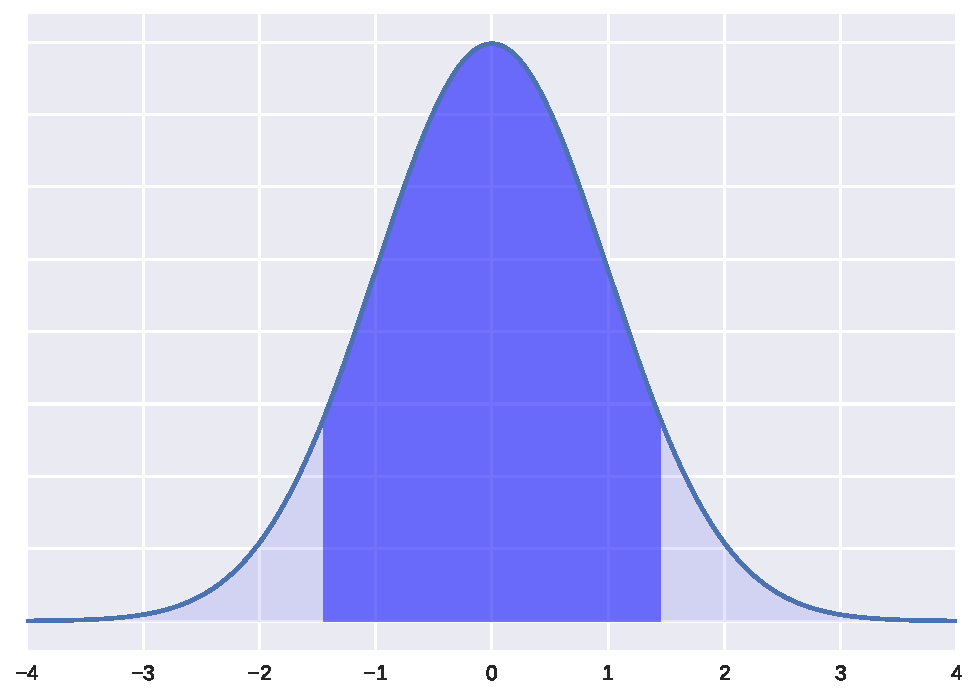
\includegraphics[width=14cm,height=7cm,keepaspectratio]{norm1f.pdf}
\centering
\end{figure}

\pagebreak

\item[g)] Between $Z = -0.90$ and $Z = 1.58$
\begin{equation*}
P(-0.90 < Z < 1.58) = \frac{1}{\sqrt{2\pi}} \int_{-0.90}^{1.58} e^{-z^{2}/2} dz = 0.75889
\end{equation*}

Program:
\lstinputlisting[language=Python]{integration1g.py}
Output:
\lstinputlisting{output11g.txt}

Program:
\lstinputlisting[language=Python]{snormscipyg.py}
Output:
\lstinputlisting{output12g.txt}

%figure_7
\begin{figure}[ht!]
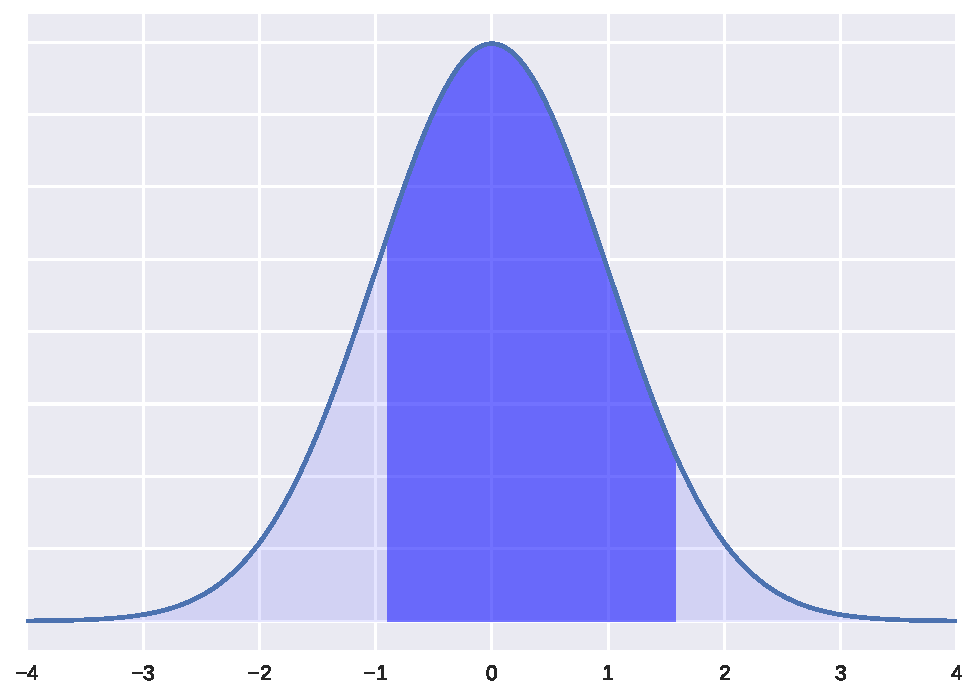
\includegraphics[width=14cm,height=7cm,keepaspectratio]{norm1g.pdf}
\centering
\end{figure}
\end{enumerate}

\pagebreak

\item[2.] The life of a certain kind of electronic device has a mean of $300$ hours and a
standard deviation of $25$ hours. Assuming that the distribution of life times which are
measured to the nearest hours can be approximated closely with a normal curve.

\vspace{1cm}

\begin{enumerate}

\item[a)] Find the probability that any one of these devices will have a lifetime of more
than $350$ hours. \\ \\
given, $\mu = 300$ and $\sigma = 25$

\begin{equation*}
\begin{split}
P(X > 350) &= \frac{1}{\sigma\sqrt{2\pi}} \int_{350}^{\infty} e^{-(x-\mu)^2/(2\sigma^{2})} dx \\
		   &= \frac{1}{25\sqrt{2\pi}} \int_{350}^{\infty} e^{-(x-300)^2/(2 \times 25^{2})} dx \\
		   &= 0.02275
\end{split}
\end{equation*}

Program:
\lstinputlisting[language=Python]{integration2a.py}
Output:
\lstinputlisting{output21a.txt}

Program:
\lstinputlisting[language=Python]{normscipy2a.py}
Output:
\lstinputlisting{output22a.txt}

\vspace{1cm}

\item[b)] What percentage will have life time from $220$ to $260$ hours?

\begin{equation*}
\begin{split}
P(220 < X < 260) &= \frac{1}{\sigma\sqrt{2\pi}} \int_{220}^{260} e^{-(x-\mu)^2/(2\sigma^{2})} dx \\
		&= \frac{1}{25\sqrt{2\pi}} \int_{220}^{260} e^{-(x-300)^2/(2 \times 25^{2})} dx \\
		&= 0.05411
\end{split}
\end{equation*}

\pagebreak

Program:
\lstinputlisting[language=Python]{integration2b.py}
Output:
\lstinputlisting{output21b.txt}

Program:
\lstinputlisting[language=Python]{normscipy2b.py}
Output:
\lstinputlisting{output22b.txt}

\end{enumerate}

\vspace{1cm}

\item[3.] The customer accounts of a certain departmental store have an average balance of
Rs.$120$ and standard deviation of Rs.$40$ Assuming that the account balances are normally
distributed, find

\vspace{1cm}

\begin{enumerate}

\item[a)] What proportion of accounts is over Rs.$150$? \\ \\
given, $\mu = 120$ and $\sigma = 40$

\begin{equation*}
\begin{split}
P(X > 150) &= \frac{1}{\sigma\sqrt{2\pi}} \int_{150}^{\infty} e^{-(x-\mu)^2/(2\sigma^{2})} dx \\
		   &= \frac{1}{40\sqrt{2\pi}} \int_{150}^{\infty} e^{-(x-120)^2/(2 \times 40^{2})} dx \\
		   &= 0.22663
\end{split}
\end{equation*}

Program:
\lstinputlisting[language=Python]{integration3a.py}
Output:
\lstinputlisting{output31a.txt}

Program:
\lstinputlisting[language=Python]{normscipy3a.py}
Output:
\lstinputlisting{output32a.txt}

\vspace{1cm}

\item[b)] What proportion of accounts is between Rs.$100$ and Rs.$150$?

\begin{equation*}
P(100 < X < 150) = \frac{1}{\sigma\sqrt{2\pi}} \int_{100}^{150} e^{-(x-\mu)^2/(2\sigma^{2})} dx 
		= \frac{1}{40\sqrt{2\pi}} \int_{100}^{150} e^{-(x-120)^2/(2 \times 40^{2})} dx 
		= 0.46484
\end{equation*}

Program:
\lstinputlisting[language=Python]{integration3b.py}
Output:
\lstinputlisting{output31b.txt}

Program:
\lstinputlisting[language=Python]{normscipy3b.py}
Output:
\lstinputlisting{output32b.txt}

\pagebreak

\item[c)] What proportion of accounts is between Rs.$60$ and Rs.$90$?

\begin{equation*}
P(60 < X < 90) = \frac{1}{\sigma\sqrt{2\pi}} \int_{60}^{90} e^{-(x-\mu)^2/(2\sigma^{2})} dx 
		= \frac{1}{40\sqrt{2\pi}} \int_{60}^{90} e^{-(x-120)^2/(2 \times 40^{2})} dx 
		= 0.15982
\end{equation*}

Program:
\lstinputlisting[language=Python]{integration3c.py}
Output:
\lstinputlisting{output31c.txt}

Program:
\lstinputlisting[language=Python]{normscipy3c.py}
Output:
\lstinputlisting{output32c.txt}
\end{enumerate}

\end{enumerate}
\end{document}
